\documentclass{sig-alternate}
\usepackage[utf8]{inputenc}
\usepackage{listings}
\usepackage{graphicx}
\usepackage{lipsum}
\usepackage{caption}
\usepackage{subcaption}
\usepackage{flushend}

\lstset{
language=Java,
basicstyle=\footnotesize,
showtabs=false, 
showspaces=false,
showstringspaces=false,
frame=single,
breaklines=true,
tabsize=2,
captionpos=b
}

\begin{document}

\conferenceinfo{MSR}{Mining Software Repositories '14}

\title{Calcuting Code Coverage Without Running the Tests:\\
A Heuristic Based on Static Code Analysis}

\numberofauthors{1}
\author{
\alignauthor
Mauricio F. Aniche, Gustavo A. Oliva, Marco A. Gerosa\\
\affaddr{Institute of Mathematics and Statistics}\\
\affaddr{University of São Paulo}\\
\email{\{aniche,goliva,gerosa\}@ime.usp.br}
}

\maketitle
\begin{abstract}

% TODO: escreve aqui o abstract? assim fica de exercicio pra ver se o texto tá claro
bla bla bla bla bla bla bla bla bla bla bla bla 
bla bla bla bla bla bla bla bla bla bla bla bla
bla bla bla bla bla bla bla bla bla bla bla bla
bla bla bla bla bla bla bla bla bla bla bla bla
bla bla bla bla bla bla bla bla bla bla bla bla
bla bla bla bla bla bla bla bla bla bla bla bla
bla bla bla bla bla bla bla bla bla bla bla bla


\end{abstract}

%%%%%%%%%%%%%%%%%%%%%%%%%%%%%%%%%%%%%%%%%%%%%%%%%%%%%%%%%%%%%%%%%%%%%%%%%%%%%%%%%%%%%%%%%%
\section{Introduction}
\label{sec:intro}

One advantage of studies that make use of mining software repository techniques
is that they can leverage a large quantity of projects and data. This huge
amount of information allows researchers to validate hypotheses with more property.

Researchers can extract data from many different sources, 
such as source code repositories (a.k.a. version control systems), 
issue trackers, mailing lists, and so on. Most of these repositories 
store textual information, which is easy to extract but hard to process. 
In the case of source code, a particular problem arises: some metrics 
require the code to be compiled first. And compiling code is a complicated task. 
Each project has its own build process and required libraries. Furthermore, 
it is common that many of these libraries are not available by the time 
researchers obtain the source code.

An example of code metric that usually requires compiled code is code coverage. 
This metric calculates the percentage of production code that is covered 
by a set of unit tests. 
Popular tools, such as Emma\footnote{http://emma.sourceforge.net/} and
Cobertura\footnote{http://cobertura.github.io/cobertura/}, instrument the code, execute
the unit test suite, and then extract the information. As said before, when dealing
with many different repositories, compiling and executing unit tests may not be
feasible.

To sort this problem out, we conceived, implemented, and evaluated a 
heuristic to calculate code coverage without compiling the code first (i.e., 
without even running unit tests). In Section \ref{sec-code-coverage}, 
we introduce the concept of code coverage. In Section \ref{sec-heuristic}, 
we present our heuristic. In Section \ref{sec-experiment}, we describe the 
experiment design. In Section \ref{sec-results}, we present the results we 
obtained and discuss them. In Section \ref{sec-threats}, 
we present the threats that may have influenced the validity of our study. 
In Section \ref{sec-related-work}, we show related studies and compare them 
to our approach. Finally, in Section \ref{sec-conclusion}, we state our 
conclusions and plans for future work.

% TODO: melhora aqui?
We found out that, although our tool implementation is not fully completed yet, the 
proposed heuristic on how to calculate code coverage using static analysis seems valid.
The maximum error on the projects evaluated was around 11\%.

%%%%%%%%%%%%%%%%%%%%%%%%%%%%%%%%%%%%%%%%%%%%%%%%%%%%%%%%%%%%%%%%%%%%%%%%%%%%%%%%%%%%%%%%%%
\section{Code Coverage}
\label{sec-code-coverage}

% TODO: tentei mostrar estudos relacionados aqiu, mas acho que poderia ter vendido melhor
Code coverage measures the quantity of production code that is being tested by
the test suite. When a unit test exercises a piece of code, developers say that the piece
of code is covered. 
Many studies argue that code coverage is an important
metric when dealing with software maintenance \cite{sebastian} \cite{del-frate} \cite{mei-hwa}.

The common output of the tools is a percentage, which is calculated
by the quantity of production code lines that are covered by at least one unit test divided by
the total number of production code lines.

There are many different ways to calculate code coverage. The tool can check the number
of lines (as mentioned before) that were executed, the number of instructions, the number of conditions, 
or even the number of executed branches.

As mentioned before, Emma and Cobertura are popular tools. 
They both use dynamic analysis to calculate the metric. They instrument the code, 
execute the unit test suite, and then discover which instructions were executed.

Besides taking a long time to calculate (as they need to execute the entire test suite),
they require compiled code. As said before, when analysing a large quantity of repositories,
compiling the code may not be an option. Researchers need an alternate way to calculate that.

%%%%%%%%%%%%%%%%%%%%%%%%%%%%%%%%%%%%%%%%%%%%%%%%%%%%%%%%%%%%%%%%%%%%%%%%%%%%%%%%%%%%%%%%%%
\section{The Proposed Heuristic}
\label{sec-heuristic}

Our heuristic is based on the idea that if a method has N different branches, then it should
have at least N different unit tests. Then, with these two numbers (branches and number of unit tests),
we calculate the ration between both. If a class contains more tests than it needs to, we round it
to 100\%.
In Table \ref{tab:ratio}, we show a few examples of combinations
and the calculated coverage. 

\begin{table}[h!]
\centering
\caption{Examples of unit tests, branches and the calculated coverage}
\begin{tabular}{ | l | l | l |}
\hline
\# of Tests & \# of Branches & Coverage in \% \\ 
\hline
10 & 10 & 100\% \\
20 & 10 & 100\% \\
10 & 0 & 0\% \\
5 & 10 & 50\% \\
7 & 10 & 70\% \\

\hline
\end{tabular}
\label{tab:ratio}
\end{table}

As we wanted to avoid dynamic analysis, the only option was to apply static analysis to
the source code. 
The first step was to estimate the number of branches a production class has. 
To do that, we decided to use McCabe's cyclomatic complexity \cite{mccabe}.
McCabe's number basically shows the different number of execution paths per method. The listing
\ref{simple-code} below exemplifies it. In that case, McCabe's number would be 2.
As we are calculating code coverage in class method, we calculate the class' cyclomatic complexity
by summing up McCabe's number of all methods.

\lstset{caption={McCabe's number to this method is 2.},
label={simple-code}}
\begin{lstlisting}
public void doSomething(int a) {
	int total = 0;
	if(a>10) total += 1;
	return total;
}
\end{lstlisting}

The next step was to count the number of unit tests that invoke a specific production method. To do that,
in a statically way, we count all the invocations that happen in the unit tests. As an example, in Listing
\ref{unit-test}, we consider the invocation to \textit{calculateTaxes()} as a unit test to it.
We then repeat this procedure to all unit tests.

\lstset{caption={An example of a unit test},
label={unit-test}}
\begin{lstlisting}
class InvoiceTest {
	@Test
	public void shouldCalculateTaxes() {
		Invoice inv = new Invoice("Customer", 5000.0);

		double tax = inv.calculateTaxes();
		double taxAgain = inv.calculateTaxes();
		
		assertEquals(5000 * 0.06, tax);
		assertEquals(5000 * 0.06, taxAgain);
	}
}
\end{lstlisting}

There are a few exception cases that are worth mentioning. 
As we are
interested in the number of distinct unit tests per production method, 
even if a test invokes the same method twice, it
counts as one. In the example above, \textit{calculateTaxes()} is invoked 
twice, but we only mark that it is being
tested by \textit{shouldCalculateTaxes()}.

Also, if a production method makes use of many other methods in its implementation,
we mark all of these methods as tested by the current unit test. In Listing \ref{calculate-taxes-impl},
we show an example of the implementation of \textit{calculateTaxes()}. In this case, we mark
methods \textit{calculateTaxes()},\textit{taxA()}, and \textit{taxB()} as tested by the 
method \textit{shouldCalculateTaxes()}, as they are all invoked by that unit test.

\lstset{caption={Internal implementation of calculateTaxes()}, label={calculate-taxes-impl}}
\begin{lstlisting}
public double calculateTaxes() {
	double taxA = taxA();
	double taxB = taxB();
	
	return taxA + taxB;
}
\end{lstlisting}

We then calculate the ratio between the number of tests and 
McCabe's number. As all metrics are calculated in method level, and we are
interested in code coverage at class level, we decided to sum up all McCabe's number and
all unit tests that test a method in that class.
In the Figure \ref{fig:formula}, we show the formula.
Again, suppose that the class \textit{Invoice} has McCabe's number equals to 10, 
and there are 6 unit tests
that invoke methods that belong to it.  
In this case, \textbf{6 / 10 = 0.6}, which means \textbf{60\%} of code coverage.

\begin{figure}[h!H]
  \centering
  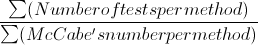
\includegraphics[scale=0.6]{imgs/formula.png}
  \caption{Formula used to calculate code coverage in our heuristic}
  \label{fig:formula}
\end{figure}

The tool that analyses the source code and calculates all of it is freely available
on Github\footnote{https://github.com/mauricioaniche/gelato2}. The all data used in this 
study is also freely available\footnote{https://github.com/mauricioaniche/msr2014}.

%%%%%%%%%%%%%%%%%%%%%%%%%%%%%%%%%%%%%%%%%%%%%%%%%%%%%%%%%%%%%%%%%%%%%%%%%%%%%%%%%%%%%%%%%%
\section{Experiment Design}
\label{sec-experiment}

To validate the heuristic, we decided to compare the code coverage calculated by it with the ones 
calculated by a dynamic analysis tool. We chose Emma as we had a previous experience with it. We
had 3 projects as subjects, all of them developed by the same company, in Java. Two of them are
web applications and one of them is a console application. In Table \ref{tab:projects}, we describe
the size of each one.

\begin{table}[h!]
\centering
\caption{Quantity of classes and methods per project}
\begin{tabular}{ | l | r | r | r | }
\hline
& Classes & Production Methods & Unit Tests\\ 
\hline
Gnarus & 769 & 1823 & 826\\ 
MetricMiner & 225 & 1009 & 341\\ 
Tubaina & 261 & 372 & 298\\ 

\hline
\end{tabular}
\label{tab:projects}
\end{table}

With both code coverage numbers (Emma's and ours), we then compared both to see how different
they were.
We used histograms and descriptive statistics. In Section below, we present the results found.

%%%%%%%%%%%%%%%%%%%%%%%%%%%%%%%%%%%%%%%%%%%%%%%%%%%%%%%%%%%%%%%%%%%%%%%%%%%%%%%%%%%%%%%%%%
\section{Findings and Discussion}
\label{sec-results}

To do the analysis, we decided to use the number calculated by our heuristic minus the
number calculated by Emma. It means that every time we find a zero, it means that both numbers
were equal, and the heuristic was perfect. A negative number indicates that the heuristic calculated
a smaller number than the real; a positive number indicates that the heuristic calculated a higher
number.

In Figure \ref{fig:metricminer}, we show the histogram of the difference between Emma and our approach to
the MetricMiner project.
In the X axis, we have the difference, 
and in the Y axis, we have the frequence.
By looking to this Figure, one can notice that most of the data are between 0 and 0.2. 
The median of the distribution is 0, and the mean is -0.1226. The first quartile is 0, and the
third quartile is also 0.

\begin{figure}[h!H]
  \centering
  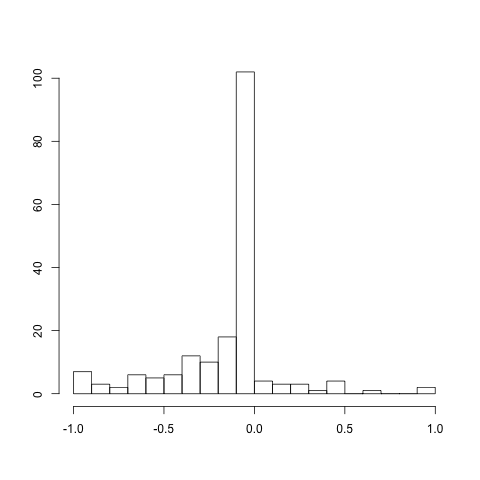
\includegraphics[scale=0.3]{../stats/metricminer-histograma-gelato.png}
  \caption{Our approach compared to Emma's in the MetricMiner}
  \label{fig:metricminer}
\end{figure}

In Figure \ref{fig:tubaina}, from Tubaina project, the data is between
0 and -0.2. However, there are a few classes that were between -0.5 and -1.0. 
The median is -0.1603, and the mean is -0.3074. The first quartile is
-0.6, and the third quartile is 0.

\begin{figure}[h!H]
  \centering
  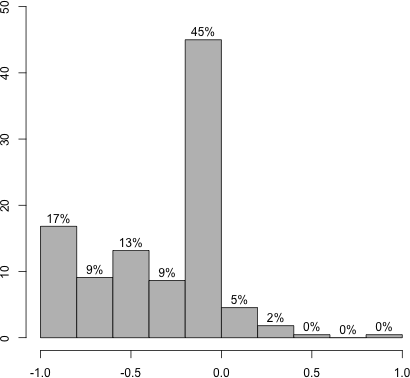
\includegraphics[scale=0.3]{../stats/tubaina-histograma-gelato.png}
  \caption{Our approach compared to Emma's in the Tubaina}
  \label{fig:tubaina}
\end{figure}


In Figure \ref{fig:gnarus}, from Gnarus project, we can see that the data is very
distributed between frequencies. The median is -0.3852, the mean is -0.3272. The first quartile
is -0.5, and the third quartile is 0.

\begin{figure}[h!H]
  \centering
  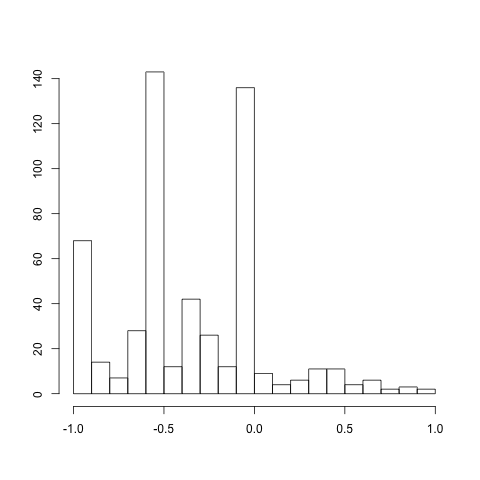
\includegraphics[scale=0.3]{../stats/gnarus-histograma-gelato.png}
  \caption{Our approach compared to Emma's in the Gnarus}
  \label{fig:gnarus}
\end{figure}

By looking to the numbers above, we notice that the heuristic was good in the first project,
in which the median was 0, regular in the second one, in which the median was -0.16. However,
in the last project, the heuristic did not go well, as the median was -0.38.

Based only on these three projects, it is hard to affirm that the heuristic is valid. However,
we decided to investigate closely on why some classes had such a bad performance. We found out
that our compiler was not interpreting a few expressions. In Listing \ref{lst:problem}, we
show an example of a misinterpreted test. In that case, the current implementation of the 
tool does not identify the invocation to \textit{doX()} and \textit{doY()} as both invocations
come from a generic list.

\lstset{caption={The tool does not identify invocations from a list}, label={lst:problem}}
\begin{lstlisting}
List<SomeClass> list = obj.getList();
assertEquals(1, list.get(0).doX());
assertEquals(1, list.get(1).doY());
\end{lstlisting}

\subsection{Isolating the heuristic}

As we identified that the implementation contains problems that are confusing the number found,
we decided to try to isolate the heuristic from the implementation. To do that, we decided to
create an aspect to the code to make it print all methods that are invoked by a unit test. After executing
the unit tests, we had an output
like the one in Listing \ref{aspectj-output}, which indicates the name of the test and the methods that were invoked.

\lstset{caption={The output produced by the aspect}, label={aspectj-output}}
\begin{lstlisting}
test com.pack1.pack2.UnitTest.testA
com.pack1.ProductionClass.methodA
com.pack1.ProductionClass.methodB
com.pack1.ProductionClass.methodC
test com.pack1.pack2.UnitTest.testB
com.pack1.ProductionClass.methodD
com.pack1.ProductionClass.methodE
\end{lstlisting}

With this information in hand, we then had the real number of unit tests per production method. We then
calculated the ratio, using McCabe's number. In Figures \ref{fig:metricminer-aj}, \ref{fig:tubaina-aj}, and
\ref{fig:gnarus-aj}, we show the histogram for MetricMiner, Tubaina, and Gnarus, respectively. 

In MetricMiner, we can notice that most of the data are between -0.2 and 0.2. 
The median of the distribution is 0, and the mean is 0.1149. The first quartile is 0, and the
third quartile is 0.2414.
In Tubaina project, the data is between
-1 and 0. The median is 0, and the mean is 0.0790. The first quartile is
0, and the third quartile is 0.1667. 
In Gnarus project, we can see that most of data
are between -2 and 0. The median is 0, the mean is -0.0152. The first quartile
is -0.7273, and the third quartile is 0.



\begin{figure}[h!H]
  \centering
  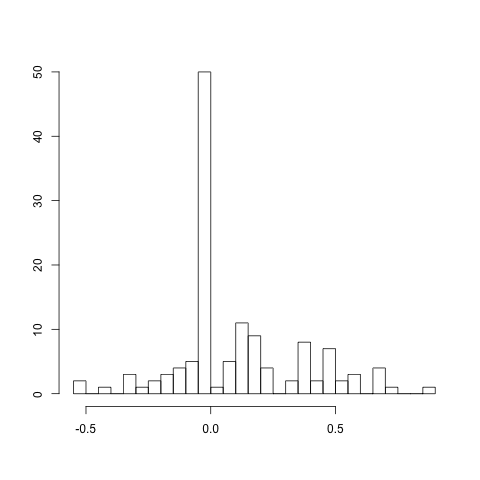
\includegraphics[scale=0.3]{../stats/metricminer-histograma-aspectj.png}
  \caption{Our second implementation compared to Emma's in the MetricMiner}
  \label{fig:metricminer-aj}
\end{figure}

\begin{figure}[h!H]
  \centering
  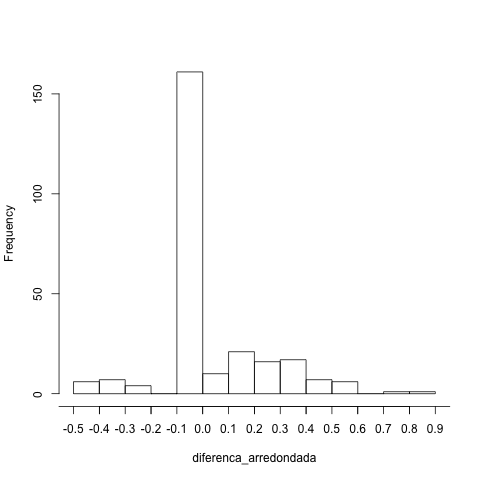
\includegraphics[scale=0.3]{../stats/tubaina-histograma-aspectj.png}
  \caption{Our second implementation compared to Emma's in the Tubaina}
  \label{fig:tubaina-aj}
\end{figure}

\begin{figure}[h!H]
  \centering
  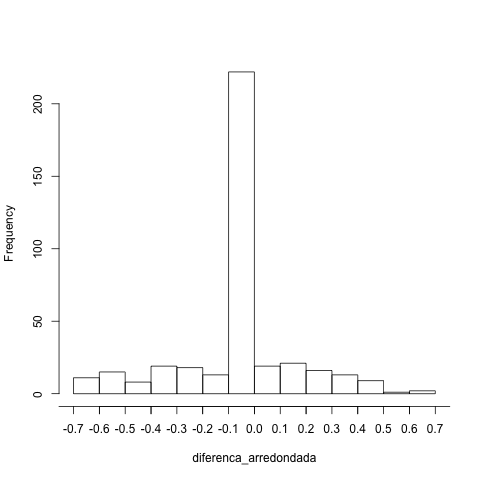
\includegraphics[scale=0.3]{../stats/gnarus-histograma-aspectj.png}
  \caption{Our second implementation compared to Emma's in the Gnarus}
  \label{fig:gnarus-aj}
\end{figure}

Based on the numbers we obtained, we believe that the heuristic has an acceptable performance. 
As the maximum mean error was 0.1149 found in these 3 projects, which means 11\%, 
we do not think that it will be a problem when using it in large software repositories.

\section{Threats to Validity}
\label{sec-threats}

There are a few threats to validity to this research. The first one is that our implementation
still does not fully work: implementing a parser is not an easy task, and one should spend
a lot of effort to completely interpret a source code. 
However, as we showed, the heuristic itself seems valid. 

We only evaluated three projects that belong to the same company. It means that these projects
follow basically the same structure, development and testing rules. That may bias the results.
In a future work, we should run the experiment in many different projects.

%%%%%%%%%%%%%%%%%%%%%%%%%%%%%%%%%%%%%%%%%%%%%%%%%%%%%%%%%%%%%%%%%%%%%%%%%%%%%%%%%%%%%%%%%%
\section{Related Work}
\label{sec-related-work}

Many studies discuss the importance of code coverage when analysing code quality. 
Sebastian et al \cite{sebastian} says that many software development practices and tools
are based on this number. However, he argues that developers usually calculate it for a single
version of the system, and perform analysis on future versions without recalculating the numbers.
He shows that even relatively small modifications on
the source code can affect the code coverage, and the impact of the change on the
metric is hard to predict.

To the best of our knowledge, there is only one study that discusses the calculation of
code coverage through static analysis.
Tiago and Visser \cite{tiago} proposes a
technique that uses slicing of static call graphs to estimate the
dynamic test coverage. 
In their approach, they define method coverage as the ratio between covered 
and defined methods per class. They showed that, at system level, the approach
proved to be satisfactory. In package and class level, the difference between
the real and the calculated coverage was small in most cases.

This approach is slightly different from ours. We use McCabe's number to estimate the
minimum number of tests a class should have. We also are more interested on calculating
code coverage in class level, while they are more worried to do it in system level. 

Also, creating a call graph is not simple. That takes more effort than just counting
the invoked methods, as we suggested.

%%%%%%%%%%%%%%%%%%%%%%%%%%%%%%%%%%%%%%%%%%%%%%%%%%%%%%%%%%%%%%%%%%%%%%%%%%%%%%%%%%%%%%%%%%
\section{Conclusion and Future Work}
\label{sec-conclusion}

% TODO: precisa melhorar tb
Code coverage is an important metric to analyse software evolution. However, it is not easy
to be calculated, as most tools require compiled code. In this study, we discuss an heuristic
to calculate it using static analysis.
Apparently, our heuristic can be used in mining software repositories studies, as the maximum
error was around 11\%.

A future work would be to run the study on more projects from different companies and 
domains.

%%%%%%%%%%%%%%%%%%%%%%%%%%%%%%%%%%%%%%%%%%%%%%%%%%%%%%%%%%%%%%%%%%%%%%%%%%%%%%%%%%%%%%%%%%
\section{Acknowledgments}

We thank Caelum Ensino and Inovação for allowing us to run the study in their environment,
as well as supporting the development of the tool.

\bibliographystyle{abbrv}
\bibliography{sigproc}

\end{document}
